%% -*- coding: utf-8 -*-
\documentclass[12pt,a4paper]{report}
\usepackage[left=2cm,right=2cm,
    top=2cm,bottom=2cm,bindingoffset=0cm]{geometry} 
\usepackage[utf8]{inputenc}
\usepackage[english,russian]{babel}
\usepackage{indentfirst}
\usepackage{misccorr}
\usepackage{graphicx}
\usepackage{amsmath}
\usepackage{amsfonts}
\usepackage{amssymb}
\setcounter{page}{2}
\begin{document}

\begin{titlepage}
\newpage
  \begin{center}
     
    Санкт-Петербургский Политехнический Университет Петра Великого \\
    
    Институт компьютерных наук и технологий \\
    
    Кафедра компьютерных систем и программных технологий
    \end{center}
    
    \vspace{15em}
    \begin{center}
    \textsc{Лабораторная работа №6}\\
    \vspace{5mm}
    \textsc{Цифровая модуляция}
    	
   \end{center}
\vspace{10em}

\newlength{\ML}
\settowidth{\ML}{«\underline{\hspace{0.7cm}}» \underline{\hspace{2cm}}}
\hfill\begin{minipage}{0.45\textwidth}
\vfill
  Руководитель \\
  \\
  \underline{\hspace{\ML}} Богач Н.\,В.\\
 
\end{minipage}%
\bigskip

\hfill\begin{minipage}{0.45\textwidth}
  Выполнил\\
  \\
  \underline{\hspace{\ML}} Солдатова Е.\,И.\\
  группа 33501/3
\end{minipage}%

\vspace{\fill}
\begin{center}
    
  Санкт-Петербург\\
   2018 
\end{center}
\end{titlepage}

\paragraph{1. Цель работы\\\\}
Изучение методов модуляции цифровых сигналов.

\paragraph{2. Постановка задачи\\}
\begin{enumerate}
\item Получить сигналы BPSK, PSK, OQPSK, genQAM, MSK, MFSK
модуляторов
\item Построить их сигнальные созвездия
\item Провести сравнение изученных методов модуляции цифровых
сигналов
\end{enumerate}

\paragraph{3. Теоретическая часть \\\\}
Множество современных коммуникационных протоколов используют квадратурную амплитудную модуляцию или QAM. Среди них, например, беспроводной Ethernet (Wi-Fi) и цифровое видео-вещание (Digital Video Broadcast (DVB)), в которых применяется модуляция 64-QAM, а также новые беспроводные технологии, такие как WiMAX и HSDPA/HSUPA (новый стандарт передачи данных в сотовой связи). QAM модуляция предназначена для передачи цифровой информации путём периодического изменения фазы и амплитуды синусоидальной электромагнитной волны. Каждая комбинация фазы и амплитуды называется символом и кодирует цифровой поток битов.

Фазовая манипуляция (phase-shift keying - PSK) является широко используемым способом цифровой модуляции, при которой данные кодируются путем изменения фазы несущего сигнала. Сигнал на несущей частоте с фазой 0 декодируется как один бит или набор битов, а с фазой 90 - как другой бит. Имеется два основных метода декодирования таких сигналов: дифференциальный и недифференциальный. Демодулятор, содержащий специальную схему PSK модуляции, может сравнивать фазу входящего сигнала с опорным сигналом или же сравнивать только изменения в фазе сигнала на несущей частоте, как это происходит при определении следующего символа.

PSK – это метод, при котором фаза несущего сигнала соответствует определенному символу. При недифференциальном кодировании на демодулятор подается опорный сигнал, который сравнивается с входящим сигналом. Разность фаз, которая сопоставляется одному символу, впоследствии, если фаза принимаемого сигнала сдвигается на какую-то величину от фазы опорного сигнала, сопоставляется другому символу или набору символов. Таким образом, фазу предыдущего символа знать необязательно. Это облегчает декодирование, так как ненужным становится механизм запоминания. Недостатком метода является необходимость включения демодулятора с опорным сигналом для выполнения сравнения.

С другой стороны, при дифференциальном декодировании можно сравнивать фазу входящего сигнала с фазой предыдущего декодированного символа. Здесь необходим механизм запоминания предыдущего символа, однако нет необходимости включения демодулятора с опорным сигналом, и мы можем игнорировать неопределённость в фазе несущего сигнала.
PSK широко применяется в различных технологиях, включая ZigBee, WiFi и радиочастотную идентификацию.

OQPSK – так обозначают манипуляцию, при которой квадратурный компонент сигнала задерживается на половину цикла. В результате компонент в фазе (I) и квадратурный компонент (Q) никогда не изменяются одновременно. Наибольшее преимущество этого факта проявляется в процессе усиления, поскольку уровень входящего сигнала практически не изменяется в промежутках между последовательными символами. Линейные усилители остаются линейными в ограниченном диапазоне амплитуд входного сигнала, и, если можно
уменьшить амплитуду, будет проще подобрать соответствующий усилитель для конкретного приложения. Кроме того, такой усилитель потребует меньше мощности, что делает его идеально подходящим для ситуаций, где используется малая мощность, как, например, в случаях с ZigBee и радиочастотной идентификацией. Лучше всего это видно при сравнении фазовых траекторий QPSK без сдвига и со сдвигом.Из рисунка видно, что траектория QPSK со сдвигом никогда не проходит через начало координат в отличие от QPSK без сдвига.

Поскольку способы PSK демодуляции несложны, при их аппаратной реализации также не возникает проблем. Например, модуляция BPSK, используемая в радиочастотной идентификации и при передаче данных в ZigBee, может быть реализована с помощью пассивных передатчиков, требующих очень малых мощностей. Так как нас интересует только фаза сигнала, основные функции для разных типов модуляции в некоторых случаях могут быть сведены к таблице соответствий, поэтому нет необходимости вычислять при помощи процессора функции sin() или cos(). Это упрощает аппаратную реализацию и программное обеспечение для цифровой обработки сигнала.

\paragraph{4. Ход работы \\\\}
Текст программы:\\\\
\%BPSK\\
signal = randi([0 1], [1 4]);\\
sig\_mod = pskmod(signal, 2);\\
scatterplot(sig\_mod);\\
sig\_demod = pskdemod(sig\_mod, 2);\\
scatterplot(sig\_demod);\\\\
\%PSK\\
signal = randi([0 7], [1 256]);\\
sig\_mod = pskmod(signal, 8);\\
scatterplot(sig\_mod);\\
sig\_demod = pskdemod(sig\_mod, 8);\\
scatterplot(sig\_demod);\\\\
\%OQPSK
signal = randi([0 2], [1 3]);\\
sig\_mod = oqpskmod(signal,8);\\
scatterplot(sig\_mod);\\
sig\_demod = oqpskdemod(sig\_mod,8);\\
scatterplot(sig\_demod);\\\\
\%genQAM\\
signal = randi([0 7], [1 256]);\\
sig\_mod = genqammod(signal, exp(j*[0:7]));\\
scatterplot(sig\_mod);\\
sig\_demod = genqamdemod(sig\_mod,exp(j*[0:7]));\\
scatterplot(sig\_demod);\\\\\\\\
\%MSK\\
signal = randi([0 1], [1 256]);\\
sig\_mod = mskmod(signal, 16);\\
scatterplot(sig\_mod);\\
sig\_demod = mskdemod(sig\_mod, 16);\\
scatterplot(sig\_demod);\\


Сигнальное созвездие BPSK (модуляция и демодуляция)

\begin{figure}[h!]
\center{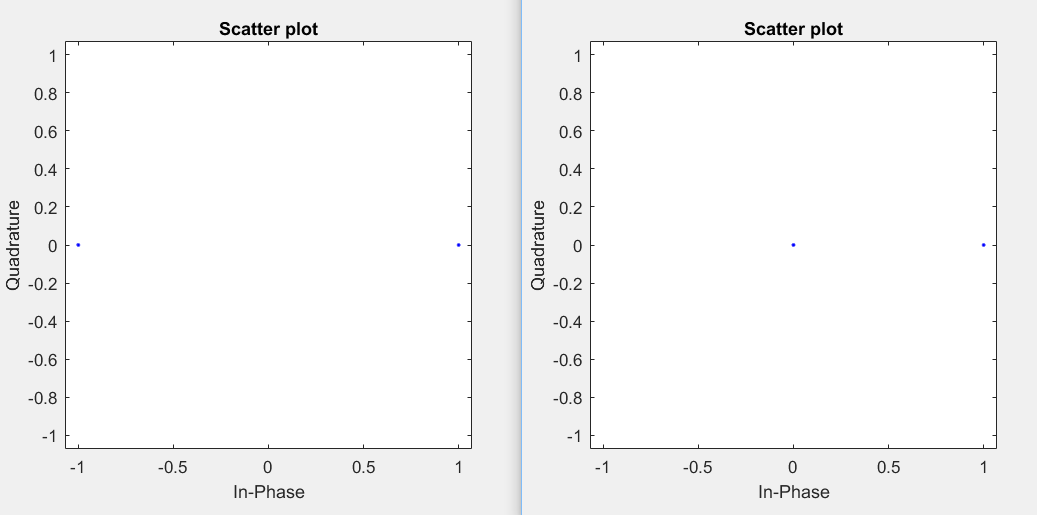
\includegraphics[width=0.7\linewidth]{bpsk}}
\end{figure}

Сигнальное созвездие PSK (модуляция и демодуляция)

\begin{figure}[h!]
\center{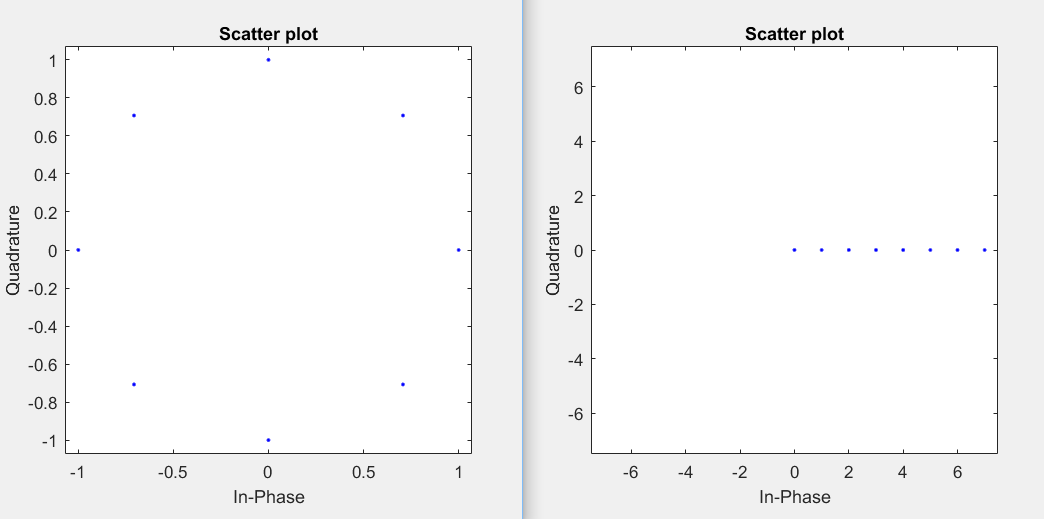
\includegraphics[width=0.7\linewidth]{psk}}
\end{figure}

Сигнальное созвездие OQPSK (модуляция и демодуляция)

\begin{figure}[h!]
\center{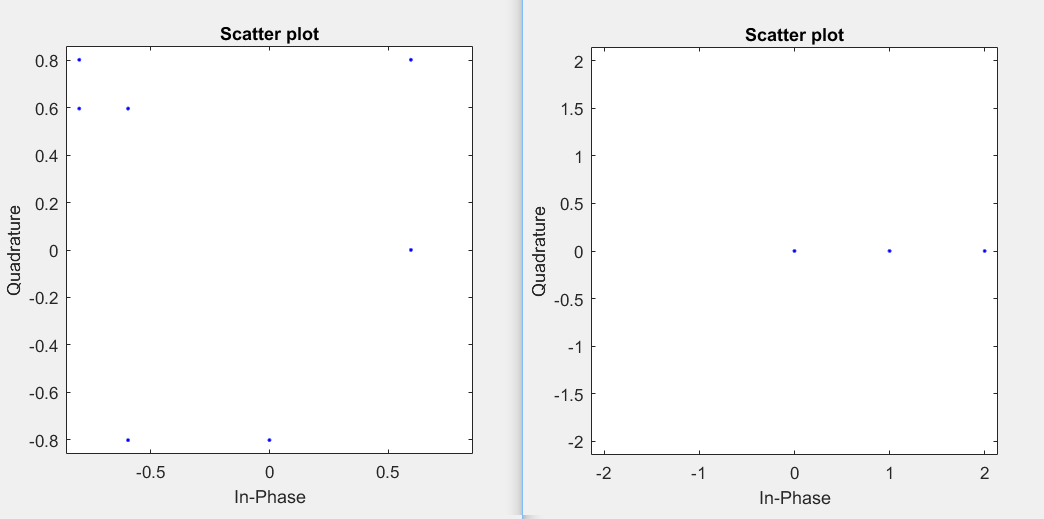
\includegraphics[width=0.7\linewidth]{oqpsk}}
\end{figure}
\newpage
Сигнальное созвездие genQAM (модуляция и демодуляция)

\begin{figure}[h!]
\center{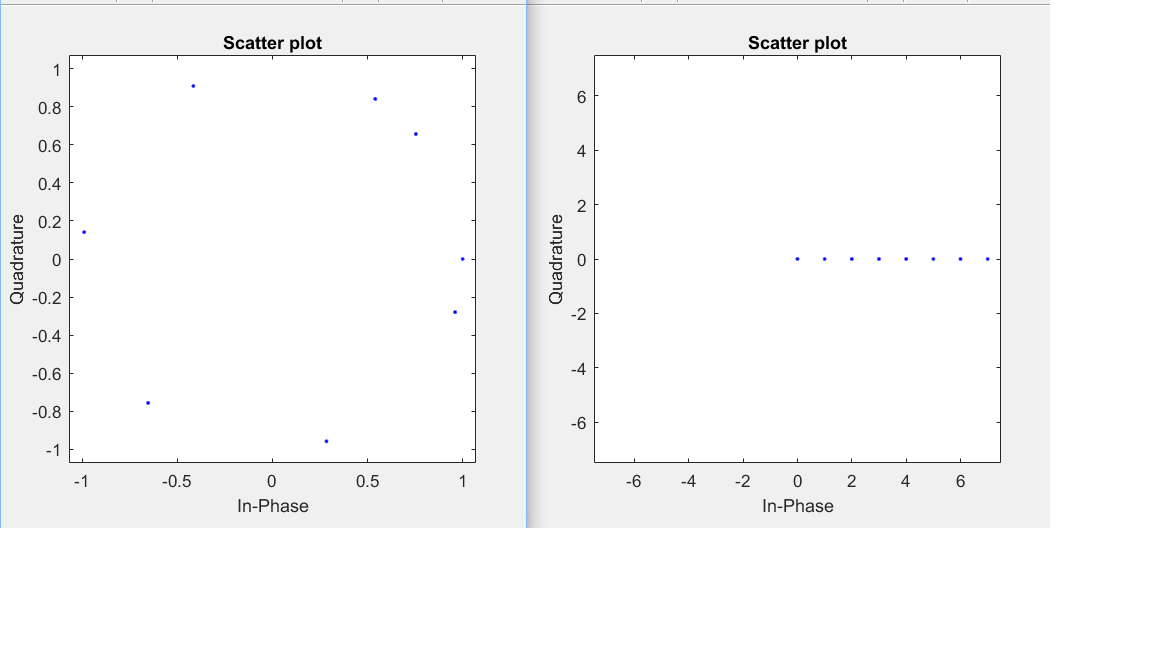
\includegraphics[width=0.7\linewidth]{genqam}}
\end{figure}

Сигнальное созвездие MSK (модуляция и демодуляция)

\begin{figure}[h!]
\center{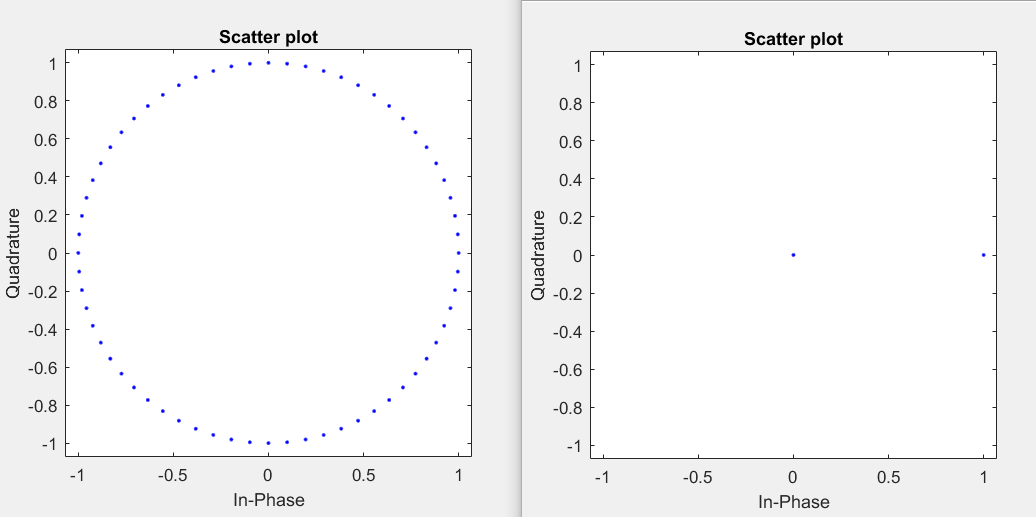
\includegraphics[width=0.7\linewidth]{msk}}
\end{figure}

\paragraph{5. Выводы \\\\}
В технике цифровой связи методы модуляции играют весьма значительную роль. Помимо своей основной функции – преобразования символ – сигнал – процесс модуляции является составной частью общего процесса согласования сигнала с характеристиками канала.

Применение многопозиционной QAM способствует передаче большего количества информации, однако в реальных усло­виях, при наличии помех, на приемной стороне возможно ошибочное определение амплитуды и фазы передаваемого сигнала. Это обстоя­тельство и ограничивает количество информации, передаваемое од­ним символом. Тем не менее, основное преимущество QAM перед другими видами модуляции — в ее хорошей помехозащищенности. Сигналы квадратурной амплитудной модуляции широко используются при передаче сигналов телевидения по радиорелейным и кабельным линиям, в системах наземного цифрового телевизионного вещания.

Способ модуляции PSK применяется в случаях, когда необхо­димо сохранить постоянной амплитуду передаваемого сигнала или исключить амплитуду из числа параметров, изменяемых в процессе модуляции. Это очень важно, например, применительно к спутниковым системам ТВ вещания.


\end{document}

